\subsection{Theoretical background}
When interpreting a language model, there is a question of what the unit of interpretability should be.
What part of the model should we be looking at?
Mechanistic interpretability aims to understand models as granularly as possible, which makes individual neurons in either the residual stream, MLP layers or attention heads the obvious choice.
Indeed, previous research has aimed to understand the behaviour and effect of individual neurons \parencite{foote_neuron_2023}\parencite{bills_language_2023}.
However, there are reasons to believe that individual neurons are fundamentally difficult to interpret.
According to the \emph{superposition hypothesis} \parencite{elhage_toy_2022}, individual neurons do not cleanly represent interpretable features.
Instead, interpretable features are spread over several neurons in order to pack more features into the same set of neuron dimensions.
This is possible due to the Johnson-Lindenstrauss lemma which implies that there are exponentially many nearly-orthogonal directions in an $n$-dimenstional space.
Therefore, by spreading out features across neurons, the model can store many more features at the cost of only a little interference.
\textcite{vaintrob_toward_2024} present a model for how the model performs computation on this representation of features.
Since features are spread over multiple neurons, this also means that each neuron represents multiple features, that it is \emph{polysemantic}.

Fortunately, even though features are not represented by individual neurons, there is some evidence for the \emph{linear representation hypothesis}.
This states that features are represented as linear combinations of neurons, i.e. directions in activation space.
\textcite{park_linear_2023} formalize the hypothesis and provide both theoretical and empirical evidence for it.
Though \textcite{engels_not_2024} show that not all features are represented in this way, much work has been done to understand the linearly represented features.
Given the linear representation hypothesis, an open problem becomes: what directions represent interpretable features?
This can be formalized as finding a transformation $\vec f\in\R^n\to\R^d$ which takes an activation vector $\vec x\in\R^n$ and gives an encoding $\vec f(\vec x)$ whose basis vectors are interpretable features.
The most studied solution to this problem, and the one we shall focus on, is that of \emph{sparse autoencoders} (SAEs).
Later, in \ref{sec:alternatives_to_saes} we will also briefly cover alternative solutions to this problem.

Apart from linearity, one of the main assumptions SAEs make is that features are \emph{sparse}.
This means that only very few features are present for each input.
\textcite{deng_measuring_2023} provide empirical evidence for both this assumption and the linear representation hypothesis.

\subsection{Sparse autoencoders}
In the context of mechanistic interpretability, SAEs  encode an activation vector $\vec x\in\R^{n}$ into a feature vector $\vec y\in\R^d$, before reconstructing $\hat{\vec x}\in\R^n$.
Autoencoders are only interesting if the feature space is somehow restricted.
In this case, that restriction comes from an $L^1$ regularization during training, which is intended to encourage sparsity and thereby hopefully polysemanticity.
The core structure of the encoder is an affine transformation followed by a ReLU nonlinearity while the decoder is simply a linear transformation \parencite{cunningham_sparse_2023}.
The loss function is the sum of mean squared error between the input and the output and the $L^1$ regularization mentioned above.
Illustration is available in figure \ref{fig:cunningham_sae_illustration} and formally this can be written as
\begin{align*}
    \vec y=&\mathrm{ReLU}\left(\mat W_e\vec x+\vec b\right)\\
    \hat{\vec x}=&\mat W_d\vec y \numberthis{eq:sae_structure}\\
    \mathcal L(\vec x)=&\norm{\vec x-\hat{\vec x}}_2^2+\alpha\norm{\vec y}_1
\end{align*}
where $\mat W_e\in\R^{d\times n}$, $\mat W_d\in\R^{n\times d}$ and $\vec b\in\R^d$ are the parameters of the model and $\alpha\in\R^+$ is a hyperparameter controlling the sparsity of the feature representation.
There are many variations to this, including in the seminal work \textcite{bricken_towards_2023} where a post-decoder bias is added that is subtracted before encoding and added after decoding.
We go into detail on some of these variations in \ref{sec:improvements_to_saes}.
As to why $L^1$ regularization recovers features, \textcite{sharkey_interim_2022} provide empirical evidence while \textcite{wright_high-dimensional_2022} provide theoretical arguments.

\begin{figure}[h]
    \centering
    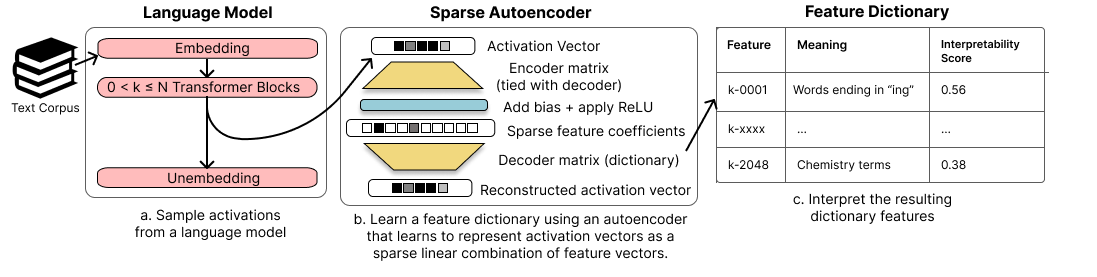
\includegraphics[width=\textwidth]{images/cunningham_sae_illustration.png}
    \caption{Borrowed from \textcite{cunningham_sparse_2023}. 
    Figure showing the structure of a SAE and its place in a language model.
    The left part of the figure shows how the input of the SAE is the activations of the language model.
    The middle part illustrates the structure of an SAE in the same way as equation \ref{eq:sae_structure}.
    $\mat W_e$ is the encoder matrix, $\mat W_d$ is the decoder matrix, $\vec b$ is the bias vector, $\vec x$ is the activation vector, and $\hat{\vec x}$ is the reconstructed activation vector and $\vec y$ is the sparse feature coefficients (latents).
    }
    \label{fig:cunningham_sae_illustration}
\end{figure}

\subsection{Improvements to sparse autoencoders}\label{sec:improvements_to_saes}
Though the performance of SAEs in the original papers \parencite{bricken_towards_2023}\parencite{cunningham_sparse_2023} was impressive, there are many ways in which they can be improved.
\textcite{taggart_prolu_2024} suggest an alternative nonlinearity to the ReLU, which they call the ProLU and is designed to overcome a theoretical weakness in using ReLU for SAEs.
They show that this improves the $L^1$/MSE Pareto frontier.
An issue that has received much attention is that of \emph{feature suppression}.
Since the loss function is the sum of the mean squared error and the $L^1$ regularization, the model is encouraged not only to activate few features, but also to keep the activations smaller than what would cause the best reconstruction.
Ideally, this would be fixed by using a $L^0$ regularization, which is what $L^1$ is a proxy for, but since $L^0$ doesn't have a gradient, this is not possible.
Instead, various other approaches have been suggested \parencite{wright_addressing_2024}.
\textcite{riggs_improving_2024} suggest taking the square root of the $L^1$ regularization term, which they show can improve the performance of the model.
This is motivated by the square root penalizing small values more than large values.
Therefore it still has the effect of encouraging sparcity, but should supress active features less.
This however does not address supression of features that are active but have low activations.
Although using an $L^0$ regularization is not possible, \textcite{rajamanoharan_improving_2024} attempt to simulate it.
They do this by separating the calculation of which features are active from that of their value.

All these represent Pareto improvements over the original SAEs according to their own experiments, but since they are tested with different methods on different models and datasets, it is hard to compare them directly.
However, \textcite{rajamanoharan_improving_2024} provide a theoretical argument for why their method should fix the same issue as the ProLU activation function along with the other advantages, so there is reason to believe that it is the best of the three.
Also, \textcite{riggs_improving_2024} only test their methods on reconstruction loss and $L^1$, so it is possible that they are overoptimizing for these and perform worse on other metrics.

Luckily, there is work that attempts to compare these methods directly.
\textcite{gao_scaling_2024} train SAEs with many of the activations suggested above along with introducing a new TopK activation function that only keeps the $k$ largest SAE latents and therefore does not need a sparsity regularization term.
Their experiments (see subsection \ref{sec:evaluation}) on GPT-4 \parencite{openai_gpt-4_2024} show that the TopK activation function performs best overall.
This result is somewhat supported by \textcite{quaisley_research_2024} which uses the methods of \textcite{huben_research_2024} to find that the a leaky TopK activation function performs best.



\subsection{Evaluation}
\label{sec:evaluation}
The last subsection touched on the issue of evaluating the performance of SAEs.
This is a difficult problem, partly because we have yet to find a good definition for interpretability, however there are some metrics that are commonly used.
The choice between them represents a tradeoff between expense and accuracy.

At the most expensive end, we have human evaluation.
This is the most accurate, since we are ultimately interested in human interpretability, but it is also the most expensive since a human must be paid to form interpretations of each individual feature.
This also makes it difficult to scale and to reproduce.
One of the most thorough examples of this can be seen in \textcite{bricken_towards_2023}.

At the other end of the spectrum, we have the $L^1$ loss used in training.
This is practically free since it is already calculated during training, but it is also a very indirect measure of interpretability.
Since we are evaluating and so do not need gradients, we can also directly measure $L^0$ loss, which is a direct measure of sparsity.
However, though there is evidence that the features we wish to find will be sparse, that does not mean that sparsity is sufficient for interpretability.
While neither of these are reliable, \textcite{bricken_towards_2023} find that they correlate sufficiently with more powerful measures to be useful as proxies during iteration.

Somewhere between these two extremes, we have automatic interpretability methods.
The most commonly used of these is that presented by \textcite{bills_language_2023}.
It consists of feeding the activations of each feature on a set of samples to a (usually different) language model and getting it to interpret the feature.
That interpretation is used by the language model to predict the activation of the feature on new samples, which can then be compared against the true activations.
How well the language model can predict the activations is then used as a measure of the quality of the interpretation.
As a measure of interpretability, it takes the quality of the LM's interpretation of the feature as a proxy of how interpretable the feature is to a human.
While being far cheaper than human evaluation, it is still expensive since it generally requires advanced language models for useful results.

A novel approach to evaluating features is presented by \textcite{makelov_towards_2024} (followup at \textcite{makelov_saes_2024}).
It suggests methods not only for evaluating the interpretability of features, but also how well they represent important parts of the model, irrespective of human interpretability.
To do this they attach attributes to samples and use these to create supervised feature dictionaries.
These are then used to benchmark unsupervised feature dictionaries, like SAEs.
It raises an important point that for many applications, human interpretability of features is not necessarily essential, as long as we can understand how to steer the model in the direction we want.
\textcite{huben_research_2024} uses evaluation methods along the same lines based on \textcite{li_emergent_2023}.
Though these methods do much to avoid dependence on the specific attributes assigned to the input, they still rely on good attributes.
This may restrict usage to cases where we know what aspects of the input we are interested in, which is part of the issue SAEs are meant to solve.
Despite this criticism, more work in the direction of finding more objective, reproduceable and scalable methods for evaluating features (on interpretability and other metrics) is sorely needed, and this is a step in the right direction.


% Introduce different methods of judging the interpretability of features by discussing papers that do so, how they do it and what they find.

% The two original papers
% Towards Principled Evaluations of Sparse Autoencoders for Interpretability and Control
% Research Report- Sparse Autoencoders find only 9 out of 180 board state features in OthelloGPT

% Loss
% Model loss when run with SAE inserted
% L0 loss (sparsity)
% Monosemanticity
% Human evaluation
%     Has to be done well. Mention interpretability illusion.
% Success of interpretability methods
%   Automatic interpretability
% Finding known features

\subsection{Applications}
\label{sec:applications}
While finding interpretable features is interesting in itself, it is not the overall goal of interpretability.
Luckily there have been many succesful attempts at using SAEs as a part of other methods.

\textcite{marks_sparse_2024} presents a fully automatic method for finding circuits \parencite{elhage_mathematical_2021} responsible for specific model behaviours.
They then manage to edit these to remove reliance on unintended signals, like gender or race.
\textcite{marks_discriminating_2024} describes how this can fit into a broader framework of scalable oversight.

\textcite{templeton_scaling_2024} and \textcite{gao_scaling_2024} explore how SAEs scale to much larger models than otherwise attempted by training SAEs on respectively Anthropics Claude 3 Sonnet \parencite{anthropic_introducing_2024} and GPT4 \parencite{openai_gpt-4_2024}.
Since the weights of neither models are open to the public, we do not know how much larger they are than previously studied models, but we do know the size of the SAEs trained on it.
While most SAEs trained in the literature have no more than 100,000 features, the SAEs trained on Claude 3 have between 1 and 34 million features and the largest SAE trained on GPT4 has 16 million latents.
This is a significant increase in scale, and the results are promising.
As with smaller SAEs, SAEs at this scale continue to find more and more nuanced features that are still interpretable.
Additionally, the work on Claude 3 show that these features can be used to steer the model in a desired direction.
Since Claude 3 is a multimodal model, they also test how the features generalize to images and find that they do so well, despite having been trained only on activations from pure text inputs.

In a similar vein, \textcite{fry_towards_2024} train an SAE directly on a vision transformer.
% Exhibits the ultra low-density cluster found in other SAEs
They find that many features are interpretable based on the highest activating samples, but also find that most features activate very rarely and seemingly rarely (what \textcite{bricken_towards_2023} call the "ultralow density cluster").
This is more than generally seen for other SAEs, but more research is required to understand whether this is a general property of vision transformer SAEs or an artifact of the authors' specific methodology.

Turning back to language models, \textcite{bloom_understanding_2024} attempt to understand features of SAEs based on logit attribution \parencite{nostalgebraist_interpreting_2020} (see \textcite{dao_adversarial_2023} for criticism), i.e. the direct effect of features on the model's output.
They split features into 4 different categories based on statistical properties of each feature's logit attribution and find that these features within each category have interesting interpretable commonalities.
However, they do not state how many features fit cleanly into each category.

While most of the work on SAEs is done on either MLP neurons or the residual stream, \textcite{kissane_sparse_2024} and \textcite{kissane_attention_2024} show that they can also be used for understanding attention layers.
In \textcite{krzyzanowski_we_2024} the same authors use the features of SAEs to study every attention head in GPT2-Small.
To do this, they find the 10 features that each head most contributes to and interpret the head based on these.
Through this methods they reproduce previous results on the roles of some heads.
They also answer an open question about the role of some of the heads and confirm with more rigorous methods that do not involve SAEs.
The reliance on the top 10 features for each head risks running into interpretability illusions \parencite{bolukbasi_interpretability_2021}, but the fact that the results line up with those from previous work and alternative methods provides evidence that this is not too severe here. 

All these applications suggest that SAEs are indeed useful both for getting a handle on what is happening inside the models and for controlling behaviour.
However, it remains to be seen whether this works in practice for models of interest.

\subsection{Criticisms}
While SAEs are surely a large step forward for interpretability, there are still many issues that must be resolved before we achieve the goals the field is working towards.
\textcite{huben_research_2024} train SAEs on OthelloGPT \parencite{li_emergent_2023} to see whether they recover the linear features found by \textcite{neel_nanda_actually_2023}.
These linear features each represent whether a specific cell has the colour of the current player and so represent the board in a human interpretable way.
However, the authors find that the SAEs only recover $9/180$ of these features.
While they do find other interpretable features, it highlights an important point that though SAEs often find interpretable features, they may not find any specific feature.

\textcite{casper_eis_2024} argues that while work on SAEs is useful, the results are often overblown.
Especially, say the authors, the work from Anthropic \parencite{bricken_towards_2023}\parencite{templeton_scaling_2024} is often presented in a way so it seems more groundbreaking than it is.
The arguments are partly based on the social media coverage surrounding the papers, but the way the Anthropic papers often focus on deep dives into a few interpretable features can make the work look more impressive.
That does not mean that it is not a method that can provide valuable insight, only that once should be wary of updating too forcefully on such possible cherry-picked examples.

Another issue that is often mentioned is the reliance on unproven proxies.
This is mentioned in many of the papers, especially those mentioned in subsection \ref{sec:evaluation}, that luckily are taking steps to resolve this issue.

As mentioned in \ref{sec:applications}, we have yet to see a concrete example of SAEs being used to solve problems in the real world, though given that the field is still young, this is perhaps to be expected.
Unfortunately, this is also connected to the issue that much of the important work of applying SAEs to real-world problems will be difficult to contribute to outside of a few large companies.
This is both due to the fact that only those companies have the resources to train SAEs of the scale required, but also because the most important work will be done on proprietary models, which are not open to the public.
This is mostly a property of the field of modern ML in general, but there may be ways to work around it, like by working on open source models like those in the Llama family \parencite{touvron_llama_nodate} and by finding ways of vastly reducing the resource requirements for training SAEs.


\subsection{Alternatives to sparse autoencoders}\label{sec:alternatives_to_saes}
% The Local Interaction Basis - Identifying Computationally-Relevant and Sparsely Interacting Features in Neural Networks
% The Singular Value Decompositions of Transformer Weight Matrices are Highly Interpretable
% Codebook Features - Sparse and Discrete Interpretability for Neural Networks
% Interpreting Neural Networks through the Polytope Lens

% Explaining Neural Networks by Decoding Layer Activations
The overall problem SAEs solve is that of finding directions in the activation space that are interpretable by humans.
SAEs are not the only proposed solution to that problem.
Instead of training a separate model to find interpretable directions in activation space, \textcite{millidge_singular_2022} looks directly at the weight matrix preceding the neurons of interest.
They take the SVD of the matrix and project it using the unembedding matrix to the token space.
Taking the top $k$ closest tokens shows that many singular vectors map to interpretable clusters of tokens.
They also show that updating the weight matrices to remove the singular vector has a larger effect on the logits for those tokens than others.
The advantage of this method is that it requires no training and is computationally far cheaper than SAEs and has fewer hyperparameters.
However, interpretation of the singular values is based solely on clusters of tokens which likely covers only a small part of interesting use-cases,
though this may be solvable by using singular vectors in other ways than the authors do.
\textcite{bushnaq_local_2024} builds on theory from \textcite{bushnaq_using_2024} to find a new activation basis.
The goal is to align the basis with the computationally important directions in order to provide an alternative but equivalent view of the model that more clearly represents the internal calculations.
When comparing to PCA on modular addition and CIFAR-10 models, they find that their method does succesfully separate the activations into features that interact sparsely, but that these results do not transfer to language models.
Both previous works differ from SAEs in that they assume (implicitly in the case of \textcite{millidge_singular_2022}) that the features of interest are not over-complete in activation space.
Given the results from work on SAEs, especially \textcite{templeton_scaling_2024}, this seems like an optimistic assumption, but since it is easier to work with and reason about fewer features, there may still be use cases for this kind of solution.

Instead of transforming existing components of the model, \textcite{tamkin_codebook_2023} inserts new components called "codebooks" into each layer.
Each added codebook consists of a set of "codes" (linear features).
For each input, the cosine similarity between each code and the input is found, and the output is the sum of the $k$ most similar codes. 
They function much like SAEs, but differ in two important ways.
Firstly, instead of encouraging sparsity with regularization, they enforce sparsity by including only some set $k$ codes.
Secondly, instead of being trained to autoencode activations after the model model has been trained, the codebook is inserted into the model from the beginning.
The first difference is interesting, since many of the issues that work presented in \ref{sec:improvements_to_saes} attempts to fix are related to precisely the $L^1$ loss, so this can be seen as a way of circumventing that entirely.
The second one however can be a large disadvantage.
There has been previous work \parencite{elhage_softmax_2022} to change the architecture of language modles to make them inherently more interpretable, but this has been largely abandoned mostly due to infeasibility \parencite{bricken_towards_2023}.
It might therefore be of interest to investigate whether codebooks can be used on pre-trained models in the same way SAEs are.


\textcite{black_interpreting_2022} provide an alternative theoretical framework for the inner workings of neural networks based on the assumption of piecewise linear activation functions.
They then \todo{should I include this?}
